\documentclass[11pt,a4paper]{article}

% Compile with LuaLaTeX. This outline preserves the shared template's visual
% style while adapting its content to EPFL CS-433 Project 1.
\usepackage[margin=1in,headheight=15pt,headsep=24pt,footskip=28pt]{geometry}
\usepackage[default]{sourcesanspro}
\usepackage{setspace}
\usepackage{xcolor}
\usepackage{mdframed}
\usepackage{titlesec}
\usepackage{fancyhdr}
\usepackage{lastpage}
\usepackage{microtype}
\usepackage{amsmath}
\usepackage{graphicx}
\usepackage{booktabs}
\usepackage[font=small,labelfont=bf]{caption}
\usepackage[hidelinks]{hyperref}

\definecolor{guidancetext}{HTML}{595959}
\definecolor{guidancebg}{HTML}{F1F3F5}

\setstretch{1}
\setlength{\parindent}{0pt}
\setlength{\parskip}{8pt}
\raggedbottom

\titleformat{\section}
  {\fontsize{14}{16.5}\selectfont\bfseries}
  {\thesection}{1em}{}
\titlespacing*{\section}{0pt}{8pt}{4pt}

\newcommand{\reporttitle}[1]{%
  {\fontsize{16}{19}\selectfont\bfseries #1\par}\vspace{10pt}%
}
\newenvironment{outlinebox}
  {\begin{mdframed}[backgroundcolor=guidancebg,linecolor=guidancebg,linewidth=0pt,
    innerleftmargin=6pt,innerrightmargin=6pt,innertopmargin=5pt,innerbottommargin=5pt,
    skipabove=5pt,skipbelow=8pt]
   \setstretch{1.0}\fontsize{9.5}{11.5}\selectfont\color{guidancetext}
   \setlength{\parskip}{3pt}}
  {\end{mdframed}}

\pagestyle{fancy}
\fancyhf{}
\renewcommand{\headrulewidth}{0pt}
\renewcommand{\footrulewidth}{0pt}
\fancyhead[L]{\fontsize{9}{11}\selectfont EPFL CS-433 Machine Learning}
\fancyhead[C]{\fontsize{9}{11}\selectfont Project 1 Report Outline}
\fancyhead[R]{\fontsize{9}{11}\selectfont Autumn 2026}
\fancyfoot[R]{\fontsize{8.5}{10}\selectfont \thepage\ (\pageref{LastPage})}

\begin{document}

\reporttitle{Predicting Cardiovascular Disease Risk from BRFSS Data}

\textbf{Team:} T123 \hfill
\textbf{Authors:} [Member 1], [Member 2], [Member 3]

\begin{outlinebox}
\textbf{Working outline -- delete guidance before submission.}
Each member first prepares an individual summary of their own work, decisions,
experiments, and results. The group will decide the final allocation later,
then merge, shorten, and harmonize the material into a maximum two-page main
report. Keep exact result values and reproducible evidence with each draft;
do not spend time polishing the final wording yet.
\end{outlinebox}

\section{Introduction and Dataset}

\begin{outlinebox}
Briefly introduce the binary classification task, the BRFSS dataset, the
\texttt{\_MICHD} target, dataset dimensions, and class imbalance. Explain why
the task is relevant and state what the project compares or aims to improve.
For the individual summary, collect the exact dataset facts and any sources
that may need to be cited; avoid a long medical background.
\end{outlinebox}

[Draft content to be inserted here.]

\section{Data Preprocessing and Feature Engineering}

\begin{outlinebox}
Summarize data cleaning and transformations: sentinel missing values,
imputation, scaling, categorical one-hot encoding, missingness indicators, and
any final feature-selection decisions. Explain the reason for each important
choice and how data leakage is avoided. In the individual summary, list which
steps were actually implemented, where they appear in the code, and any
measured effect on validation performance.
\end{outlinebox}

[Draft content to be inserted here.]

\section{Models and Validation Protocol}

% This contribution covers one of the team's three methods only.
\textbf{3.1 L2-regularized logistic regression.}
Before fitting this model, we used an 80/20 stratified train/validation split
(seed 42). Preprocessing was fitted on the training split only: all-missing
and constant columns were removed, remaining missing values were replaced
with training medians, and features were standardized using training means
and standard deviations. This retained 315 of 321 input features. All six removed columns were constant in this split. Survey
codes were kept as numerical inputs; sentinel recoding and one-hot encoding
were not applied.

We implemented logistic regression in NumPy, with score
$p_i=\sigma(\mathbf{x}_i^\top\mathbf{w}+b)$, minimizing mean binary
cross-entropy plus $\lambda\lVert\mathbf{w}\rVert_2^2$; the intercept was
not penalized. All 23,180 positive training examples were retained and an
equal number of negatives were randomly sampled once before optimization.
Mini-batch gradient descent used 20 epochs, batch size 2,048,
$\lambda=10^{-4}$, and learning rate
$\eta_e=0.1/\sqrt{1+e/5}$ for epochs $e=0,\ldots,19$.

The 65,627 validation examples kept their original class proportions.
With training settings fixed, we compared thresholds maximizing accuracy,
balanced accuracy, and positive-class F1. Accuracy and balanced accuracy
were searched on a 0.005 grid; F1 was evaluated at every distinct validation
score, also including 0 and 1. We report the F1-selected configuration as
this method's F1-oriented candidate, rather than a final team-wide choice.
The same split is used for threshold selection and reporting, so these are
tuning results rather than an independent estimate of generalization.

\textbf{3.2 Class-weighted linear SVM.}
We used the same 80/20 stratified split and seed 42. In contrast to the basic
numeric preprocessing above, the SVM used the BRFSS codebook to convert
feature-specific ``Don't know'' and ``Refused'' codes to missing values.
Numeric variables were median-imputed and standardized, numeric missingness
indicators were added, and categorical variables were one-hot encoded with a
separate missing category. All preprocessing parameters were fitted on the
training partition only, yielding 1,194 features including the intercept.

The NumPy-only linear soft-margin SVM minimized the class-weighted objective
\begin{equation}
  \frac{1}{N}\sum_{i=1}^{N}\alpha_i
  \max\!\left(0,1-y_i\mathbf{w}^{\top}\mathbf{x}_i\right)
  +\frac{\lambda}{2}\lVert\mathbf{w}\rVert_2^2,
\end{equation}
where $\alpha_i=N_-/N_+=10.3248$ for positive examples and $1$ otherwise.
Stochastic subgradient descent used $\lambda=0.01$, learning rate $10^{-4}$,
200,000 updates, and seed 42. We evaluated 302 thresholds derived from the
validation decision scores, also including the standard SVM threshold zero.
The F1-oriented candidate was selected by maximum positive-class F1, with
balanced accuracy used only as a tie-break. As for logistic regression,
threshold selection and reporting use the same validation split.

\textbf{3.3 Method 3.} [To be completed by the responsible team member.]

\newpage

\section{Results}

\textbf{4.1 Logistic regression: threshold selection.}
% Values below are regenerated from outputs/*_validation.json.
% This is one fitted method evaluated at three thresholds, not three models.
Table~\ref{tab:lr-thresholds} and Figure~\ref{fig:lr-thresholds} compare three
operating points of the same model. Maximizing F1 selected a threshold of
0.737053: validation F1 increased from 0.110 to 0.414 relative to the
accuracy-selected threshold, while accuracy decreased from 91.3\% to
87.1\%. Recall increased from 6.11\% to 51.65\%. Lowering the threshold
further to maximize balanced accuracy increased recall to 83.3\%, but
reduced precision to 22.4\% and F1 to 0.353. Thus, the threshold objective
substantially changes minority-class detection without changing the model
weights.

\begin{table}[htbp]
\centering\small
\caption{Local validation results for one logistic regression model.
Scores are rounded; F1 refers to the positive class.}
\label{tab:lr-thresholds}
\begin{tabular}{lrrrrr}
\toprule
Threshold objective & Threshold & Accuracy & Precision & Recall & F1 \\
\midrule
Accuracy & 0.940 & 0.913 & 0.567 & 0.061 & 0.110 \\
Balanced accuracy & 0.470 & 0.731 & 0.224 & 0.833 & 0.353 \\
F1 & 0.737 & 0.871 & 0.345 & 0.516 & \textbf{0.414} \\
\bottomrule
\end{tabular}
\end{table}

\begin{figure}[htbp]
\centering
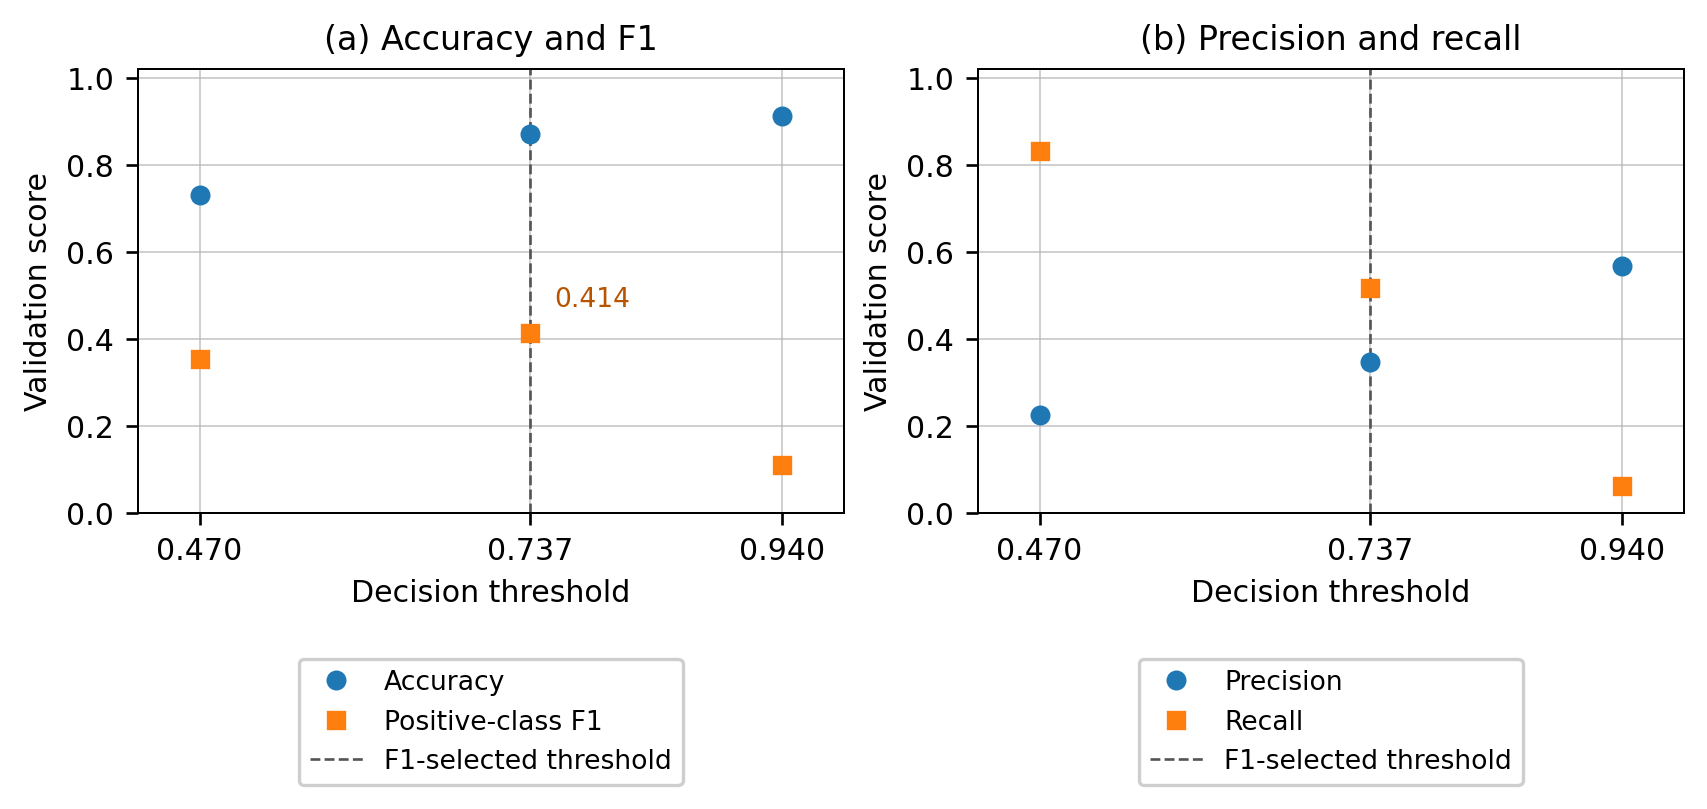
\includegraphics[width=\linewidth]{logistic_threshold_results.png}
\caption{Validation performance at the three selected logistic-regression
thresholds. Markers show measured operating points; the dashed line identifies
the F1-selected threshold. No values between the recorded points are inferred.}
\label{fig:lr-thresholds}
\end{figure}

\textbf{4.2 Linear SVM: decision-threshold selection.}
At the standard SVM threshold zero, the model obtained 0.806 accuracy, 0.771
balanced accuracy, 0.729 recall, and 0.399 F1. Maximizing validation F1 selected
a decision-score threshold of 0.5009. This reduced false positives from 11,147
to 6,126 and increased precision from 0.275 to 0.349. The resulting accuracy
was 0.868 and F1 was 0.432, while recall decreased from 0.728 to 0.566 and
balanced accuracy from 0.771 to 0.732. Figure~\ref{fig:svm-thresholds} therefore
shows the expected precision--recall trade-off rather than a uniformly better
operating point.

\begin{figure}[htbp]
\centering
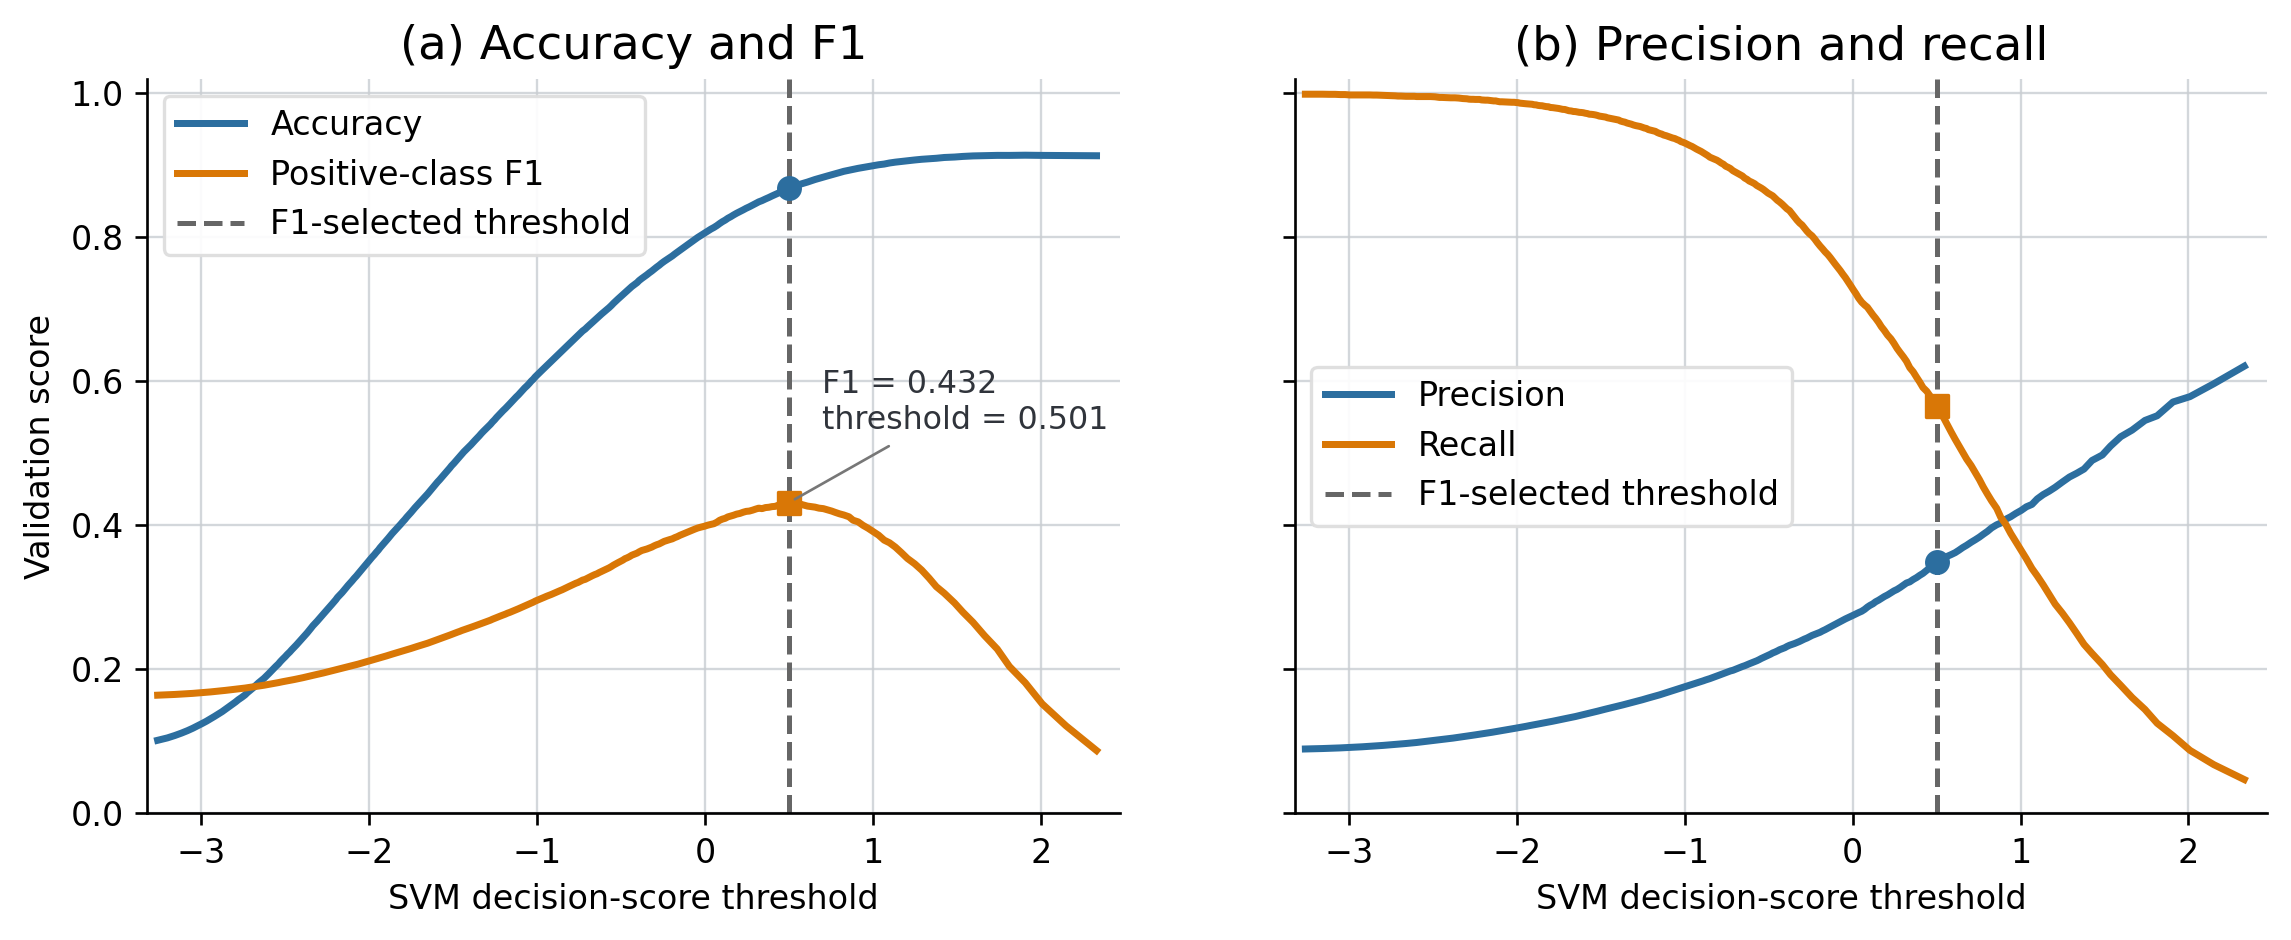
\includegraphics[width=\linewidth]{svm_threshold_results.png}
\caption{Validation performance of the class-weighted linear SVM across real
decision-score thresholds. Curves are computed from the same validation scores;
the dashed line marks the threshold maximizing positive-class F1.}
\label{fig:svm-thresholds}
\end{figure}

\textbf{Three-method comparison (pending team results).}
The rows below use each completed method's F1-selected threshold. Method 3 and
the final team-wide choice remain pending.

\begin{center}\small
\begin{tabular}{lrrrr}
\toprule
Method & Accuracy & Balanced acc. & F1 & Recall \\
\midrule
L2 logistic regression (F1 threshold) & 0.871 & 0.711 & 0.414 & 0.516 \\
Weighted linear SVM (F1 threshold) & 0.868 & 0.732 & \textbf{0.432} & 0.566 \\
Method 3 & -- & -- & -- & -- \\
\bottomrule
\end{tabular}
\end{center}

These are local validation scores. The all-negative reference achieves 91.17\%
accuracy but zero positive-class F1 and recall. On AIcrowd, the SVM at threshold
zero obtained F1 0.401 and accuracy 0.804, whereas the F1-selected threshold
0.5009 obtained F1 0.431 and accuracy 0.866.

\section{Discussion}

The completed methods show that threshold choice matters almost as much as the
linear model family under strong class imbalance. At their locally F1-selected
operating points, the SVM achieved slightly higher F1, balanced accuracy, and
recall than logistic regression, whereas logistic regression achieved slightly
higher ordinary accuracy. The SVM's class weighting and codebook-aware one-hot
representation improved minority-class detection, but this comparison also
mixes modeling and preprocessing differences. A final claim about the best
algorithm therefore requires Method 3 and, ideally, a common preprocessing
ablation. The close match between the threshold-selected SVM's local scores and
its AIcrowd result provides some evidence that the shared holdout is representative.

\begin{outlinebox}
Interpret the most important comparisons rather than repeating the table.
Discuss the effects of preprocessing and class weighting, the trade-off between
accuracy and positive-class detection, and the agreement between local
validation and AIcrowd performance. Individual summaries should contribute two
or three evidence-backed observations, including unsuccessful choices when
they help explain the final design.
\end{outlinebox}

\section{Limitations and Conclusion}

The logistic and SVM thresholds were selected and reported on the same
validation split, so their F1 values are tuning estimates rather than fully
independent generalization estimates. Repeated cross-validation or a final
untouched holdout would better quantify this uncertainty. The BRFSS labels and
predictors are self-reported, missingness is substantial, and the class-weighted
SVM sacrifices precision to detect more positive cases. Finally, the current
comparison does not isolate the effect of model choice from preprocessing.

\begin{outlinebox}
State the main limitations concisely, including self-reported survey data,
class imbalance, missingness, and validation uncertainty. Distinguish limits
of the dataset from limits of the modeling procedure. Finish with the main
result and one realistic improvement. Each individual summary should propose
at least one limitation and one feasible next step for the group to discuss.
\end{outlinebox}

\section*{References}

[Add only sources cited in the final report, using one consistent style.]

\end{document}
